\section{THE BOUNDARY VALUE PROBLEM}

This section discusses the mathematical formulation of the BVP for CTCRs. It introduces the Cosserat rod model, examines the stiffness of the model, and reviews existing methods, setting the foundation for the computational benchmarks explored later.

\commentblock{
\begin{table}[thb!]
	\centering
	\caption*{\textsc{Nomenclature}}
	\label{tab:nomenclature}
    \resizebox{0.49\textwidth}{!}{%
        \begin{tabular}{l l}
            \hline
            \hline
            \\
    
            $\boldsymbol{a}$      & \text{Bold typeface for vectors} \\
            $A$                   & \text{Uppercase typeface for matrices} \\
            $n$                   & \text{Number of concentric, precurved tubes} \\
            $s$                   & \text{Point along the robot's arc-length} \\
            $(\cdot)^*$           & \text{Denotes that the variable is in the undeformed state} \\
            $\boldsymbol{r}_i(s)$ & \text{The position vector for tube $i$ at point $s$} \\
            $R_i(s)$              & \text{The rotation matrix for tube $i$ at point $s$} \\
            $g_i(s)$              & \text{The reference frame for tube $i$ at point $s$} \\
            $E_i$                 & \text{Young's modulus for tube $i$} \\
            $G_i$                 & \text{Shear modulus for tube $i$} \\
            $I_i$                 & \text{The second moment area for tube $i$} \\
            $J_i$                 & \text{The polar moment of inertia of the $i$th tube's cross-section} \\
            $K_i$                 & \text{Stiffness matrix for tube $i$} \\
            $(\cdot)^\vee$        & \text{Denotes the conversion from $\mathfrak{so}(3)$ or $\mathfrak{se}(3)$ to $\mathbb{R}^3$ or $\mathbb{R}^6$ respectively} \\
            $\widehat{\cdot}$     & \text{The inverse function of $(\cdot)^\vee$} \\
            $\boldsymbol{u}_i(s)$ & \text{Precurvature vector for tube $i$ at point $s$} \\
            $\theta_i$            & \text{Axial angle of the $i$th tube} \\
            $\boldsymbol{\xi}$    & \text{Rate of change of the reference frame $g$} \\
            $u_{i,z}(s)$          & \text{Torsional strains for tube $i$ at point $s$} \\ 
            $\alpha_i$            & \text{Rotational joint value corresponding to the $i$th tube} \\
            $\beta_i$             & \text{Translational joint value corresponding to the $i$th tube} \\
            $\boldsymbol{q}$      & \text{The robot's joint space vector} \\
            $L_i$                 & \text{Length of the $i$th tube} \\
            $\boldsymbol{y}$      & \text{State vector for the ODE system} \\
            $\boldsymbol{f}(s, \boldsymbol{y})$ & \text{Derivative of the state vector} \\
            $A(s)$                & \text{Jacobian matrix of the ODE system at point $s$} \\
            $\lambda_j(s)$        & \text{Eigenvalue of $A(s)$} \\
            $h$                   & \text{Integration step-size} \\
            $k$                   & \text{Non-linear solver iteration count} \\
            $n_{\boldsymbol{f}}(h)$              & \text{Denotes the number of calls to $f$ using a step-size of $h$} \\
            $e_p$                 & \text{Position error} \\
            
            \\
            \hline
            \hline
        \end{tabular}
    }
\end{table}
}

\subsection{The Cosserat Rod Model}

\bulletpoints{
    \item Topic Sentence: A brief overview of Cosserat Rod theory. This paragraph should discuss the forces it models and the simplifying assumptions made by Kirchhoff and by us in this paper.
    \item Introduce Cosserat Rod theory
    \item Cosserat Rod theory uses bend, twist, stretch, and shear to represent the 6 dof
    \item Introduce Kirchhoff assumptions
    \item Discuss our own assumptions (Constant precurvature and precurved around x-axis)
}

\commentblock{
Cosserat rod theory provides a comprehensive mathematical framework for modeling slender, one-dimensional rods by accounting for bend, twist, stretch, and shear to represent all six degrees of freedom at each cross-section \cite{RuckerJonesWebster_TRO_2010}.
In the context of CTCRs, Kirchhoff rod theory, a special case of Cosserat rod theory that assumes inextensibility and shearlessness, is used.
These assumptions are generally valid given the long, thin Nitinol tubes used in CTCRs \cite{RuckerJonesWebster_TRO_2010}.
In addition to the Kirchhoff assumptions, we will further assume that the tubes' precurvature is constant across the arc length and that the tubes are precurved solely around the x-axis as is shown in Fig.~\ref{fig:ctcr}.
}

\bulletpoints{
    \item Topic Sentence: Walk through the Cosserat Rod equations and explain how it gives rise to the ODE system.
    \item Explain how the reference frames are formed
    \item Introduce the stiffness matrix and local precurvature vector
    \item Explain how to initialize the state variables
    \item Introduce the final ODE system which forms the BVP
    \item Introduce the initial and final boundary conditions
}

\commentblock{
To model a collection of $n$ concentric, precurved tubes, we must assign homogeneous reference frames along the tubes' arc-lengths.
By convention, the $z$-axes of these frames are always tangent to the curve of the tube, resulting in the frame formulation
\begin{align*}
    g^{*}_i(s) =
    \begin{bmatrix}
		R^{*}_i(s) & \boldsymbol{r^{*}_i}(s)\\
		\boldsymbol{0}^T & 1\\
	\end{bmatrix}
    .
\end{align*}
The material properties and the tube's geometry of each cross-section can be described by the stiffness matrix $K_i$ and the local precurvature vector $\boldsymbol{u}_i(s)$ respectively:
\begin{align*}
    & K_i =
    \begin{bmatrix}
		E_iI_i & 0 & 0\\
		0 & E_iI_i & 0\\
        0 & 0 & G_iJ_i\\
	\end{bmatrix},
    & \boldsymbol{u}^{*}_i(s) =
    \begin{pmatrix}
		R^{*T}_i(s)\dot{R}^{*}_i(s)
	\end{pmatrix}^\vee &
    .
\end{align*}
Lastly, by initializing the following state variables as
\begin{align*}
    & R_{\theta_i} = \begin{bmatrix}
		\cos \theta_i & -\sin \theta_i & 0\\
		\sin \theta_i & \cos \theta_i & 0\\
        0 & 0 & 1\\
	\end{bmatrix} & K = \sum^n_{i = 1} K_i \\
    & \boldsymbol{u}_i = R^T_{\theta_i}\boldsymbol{u}_1 + \dot{\theta}_i \boldsymbol{e}_3 & \boldsymbol{\xi} = \begin{bmatrix}
		0 & 0 & 1 & \boldsymbol{u}^T_1\\
	\end{bmatrix}^T
    ,
\end{align*}
an ODE system can be constructed using the Cosserat rod equations to describe the tubes' shapes along with the elastic interactions between them:
\begin{align*}
    \dot{g} &= g\widehat{\boldsymbol{\xi}}\\
    \dot{\theta}_i &= u_{i, z} - u_{1, z}\\
    \begin{bmatrix}
		\dot{u}_{1, x}\\
		\dot{u}_{1, y}\\
	\end{bmatrix} &= -K^{-1}(\sum^{n}_{i=1} R_{\theta_i}(K_i (\dot{\theta}_i \frac{dR^T_{\theta_i}}{d\theta_i}\boldsymbol{u}_1) \\
    & + \widehat{\boldsymbol{u}}_i K_i (\boldsymbol{u}_i - \boldsymbol{u}^{*}_i)) + \widehat{e}_3 R^T_1 \boldsymbol{w}_f)|_{x, y}\\
    \dot{u}_{i, z} &= \frac{E_iI_i}{G_iJ_i}(u_{i, x}u^{*}_{i, y} - u_{i, y}u^{*}_{i, x})
    .
\end{align*}
With constant tube precurvature and zero z-axis curvature, the final boundary condition simplifies to zero torsional strains $u_{i, z}$ at each tube's end.
The initial boundary condition at $s = 0$ relates to the robot's joint space and is defined as:
\begin{align*}
    & \boldsymbol{r}(0) = \begin{bmatrix}
		0 & 0 & 0\\
	\end{bmatrix}^T & \theta_1 = \alpha_1 - \beta_1 u_{1, z} \\
 & \theta_i = (\alpha_i - \beta_i u_{i, z}) - \theta_1, \quad i \geq 2
 .
\end{align*}
}

\subsection{Stiffness Analysis of the BVP}

\bulletpoints{
    \item Topic Sentence: Define the ODE system and the jacobian matrix $A(s)$. Briefly explain BVP stiffness.
    \item Define $A(s)$ using $f(s, y)$ and using the state variables
    \item Introduce the BVP criterion for stiffness
    \item Compare BVP stiffness to IVP stiffness and explain the effect of boundary conditions on solution divergence.
    \item Establish the need to determine an upper bound for the eigenvalues.
}

\commentblock{
\begin{figure*}[t!]
    \normalsize

    \begin{align*}
        A(s) = \begin{bmatrix}
                0 & \cdots & 0 & 0 & 0 & -1 & 1 & \cdots & 0\\
                \vdots & \ddots & \vdots & \vdots & \vdots & \vdots & \vdots & \ddots & \vdots\\
                0 & \cdots & 0 & 0 & 0 & -1 & 0 & \cdots & 1\\
                \frac{\partial f_n}{\partial y_1} & \cdots & \frac{\partial f_n}{\partial y_{n-1}} & \frac{\partial f_n}{\partial y_n} & \frac{\partial f_n}{\partial y_{n+1}} & \frac{\partial f_n}{\partial y_{n+2}} & \frac{\partial f_n}{\partial y_{n+3}} & \cdots & \frac{\partial f_n}{\partial y_{2n+1}} \\
                \frac{\partial f_{n+1}}{\partial y_1} & \cdots & \frac{\partial f_{n+1}}{\partial y_{n-1}} & \frac{\partial f_{n+1}}{\partial y_n} & \frac{\partial f_{n+1}}{\partial y_{n+1}} & \frac{\partial f_{n+1}}{\partial y_{n+2}} & \frac{\partial f_{n+1}}{\partial y_{n+3}} & \cdots & \frac{\partial f_{n+1}}{\partial y_{2n+1}} \\
                0 & \cdots & 0 & \frac{\partial f_{n+2}}{\partial y_n} & \frac{\partial f_{n+2}}{\partial y_{n + 1}} & 0 & 0 & \cdots & 0 \\
                \frac{\partial f_{n+3}}{\partial y_1} & \cdots & 0 & \frac{\partial f_{n+3}}{\partial y_n} & \frac{\partial f_{n+3}}{\partial y_{n + 1}} & 0 & 0 & \cdots & 0 \\
                \vdots & \ddots & \vdots & \vdots & \vdots & \vdots & \vdots & \ddots & \vdots\\
                0 & \cdots & \frac{\partial f_{2n+1}}{\partial y_{n-1}} & \frac{\partial f_{2n+1}}{\partial y_n} & \frac{\partial f_{2n+1}}{\partial y_{n + 1}} & 0 & 0 & \cdots & 0 \\
        \end{bmatrix}
    \end{align*}

    \caption*{The analytical Jacobian of the non-linear ODE presented in Eq.~\ref{eq:ode_system}.}
    \label{eq:analytical_Jacobian}
\end{figure*}

The stiffness of an ODE system indicates its conditioning.
Stiff ODEs require the use of implicit integrators and/or minuscule step sizes to prevent divergence, while non-stiff ODEs allow the use of explicit integrators with moderate step sizes \cite{AscherPetzold_SIAM_1998, Heath_SIAM_2018}.
Consider the BVP described by the following non-linear ODE system
\begin{align}
    \label{eq:ode_derivative}
    \dot{\boldsymbol{y}} = \boldsymbol{f}(s, \boldsymbol{y}), \quad 0 \leq s \leq b\\
    A(s) = \frac{\partial \boldsymbol{f}}{\partial \boldsymbol{y}}(s, \boldsymbol{y})
    \label{eq:ode_system}
    ,
\end{align}
where $A(s) \in \mathbb{R}^{m \times m}$.
A BVP is considered stiff if and only if
\begin{align*}
    b|\Re(\lambda_j(s))| \gg 1, \quad 1 \leq j \leq m
    ,
\end{align*}
\cite{AscherPetzold_SIAM_1998}.
Unlike IVPs, BVP stiffness depends on boundary conditions, allowing it to tolerate error accumulation from positive eigenvalues if the integration interval near the final boundary $b$ is small enough \cite{AscherPetzold_SIAM_1998}.
}

\bulletpoints{
    \item Topic Sentence: Lay down the foundations for the statistically derived upper-bound.
    \item Define the state vector for the ODE system
    \item Finding an analytical upper bound is tough, that is why we sampled 20 million configurations.
    \item The The configurations were sampled uniformly and the maximum over the interval was calculated
}

\commentblock{
Following \cite{RuckerWebster_ICRA_2011}, we define our state $\boldsymbol{y}$ as
\begin{align}
    \boldsymbol{y} &= [\theta_2, \cdots, \theta_n, u_{1, x}, u_{1, y}, u_{1, z}, u_{2, z}, \cdots, u_{n, z}]^T\\
	&= [y_1, \cdots, y_{n - 1}, y_n, y_{n + 1}, y_{n + 2}, y_{n + 3}, \cdots, y_{2n + 1}]^T
    \label{eq:state_variables}
\end{align}
where the first $n - 1$ elements determine the position and orientation at $s$, and the remaining elements describe tube bending and torsion \cite{RuckerJonesWebster_TRO_2010}.
Deriving an analytical upper bound for the eigenvalues of $A(s)$ is challenging due to the non-linear relationships between the state variables.
Instead, we employed a statistical approach, sampling $20,000,000$ configurations uniformly and calculating the maximum $max(|\Re(\lambda_j(s))|)$ across the integration interval. 
}

\bulletpoints{
    \item Topic Sentence: Discuss the upper-bound used and how it satisfies the criterion.
    \item The upper bound used is 20 because it is really improbably that the eigenvalues will be higher.
    \item Using 20 as the upper bound and b = 0.21, the criterion is satisfied.
    \item Yeah, this might seem sketchy but it is safe to assume it's not
}

\commentblock{
\begin{figure}
    %\fbox{
    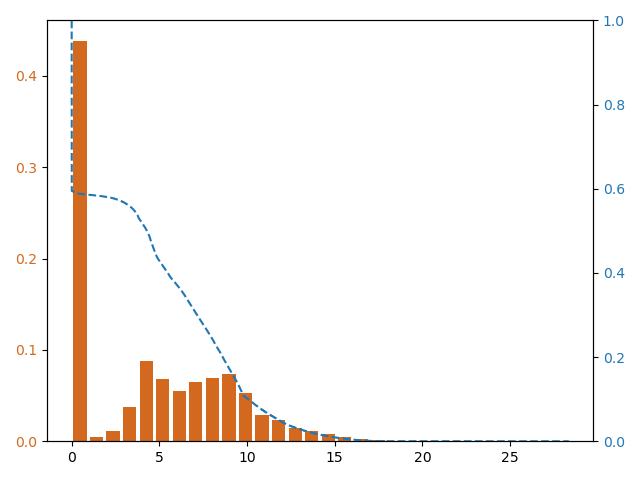
\includegraphics[width=\columnwidth]{Figures/max eigen_histogram.png}
    %}
    \caption{
    Histogram of the sampled $max(|\Re(\lambda_j(s))|)$. The orange bars represent the density while the blue line represents the empirical complementary cumulative distribution function (CCDF). A total of $20,000,000$ configurations were sampled.
    }
    \label{fig:eigen_distribution}
\end{figure}

We use $20$ as the upper bound for the system's eigenvalues since $|\Re(\lambda_j(s))| > 20$ has only a $0.001\%$ probability of occurrence, as can be seen in Fig. ~\ref{fig:eigen_distribution}.
With a maximum CTCR arc length of 210 mm, we assume
\begin{align*}
    0 \leq |\Re(\lambda_j(s))| \leq 20\\
    0 \leq b|\Re(\lambda_j(s))| \leq 4.2
\end{align*}
where $b=0.21$, indicating that the BVP is non-stiff.
While the aforementioned, approximated eigenvalue upper-bound is specific to the CTCR parameters used, the widespread success of using the shooting method with the explicit classical Runge-Kutta integrators \cite{Burgner-Kahrs_TRO_2015} suggests that the BVP is generally non-stiff.
}